\documentclass{standalone}
\usepackage{tikz}
\begin{document}
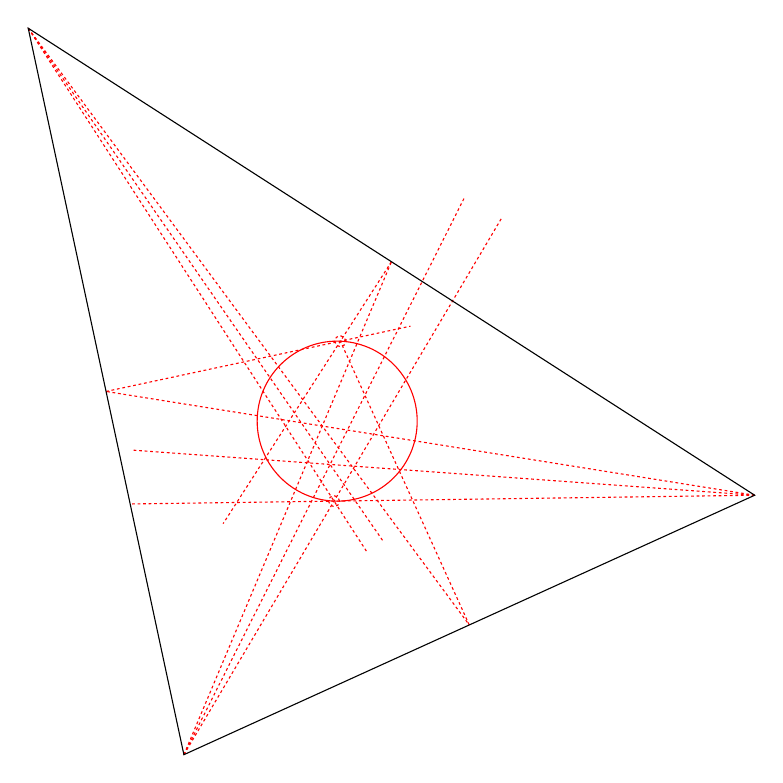
\begin{tikzpicture}[x=1pt,y=1pt]
\draw[red, dash pattern=on 1pt] (18.75,-18.75) -- (178.12,-234.38);
\draw[red, dash pattern=on 1pt] (281.25,-187.50) -- (46.88,-150.00);
\draw[red, dash pattern=on 1pt] (75.00,-281.25) -- (150.00,-103.12);
\draw[red, dash pattern=on 1pt] (18.75,-18.75) -- (146.77,-203.77);
\draw[red, dash pattern=on 1pt] (281.25,-187.50) -- (56.85,-171.23);
\draw[red, dash pattern=on 1pt] (75.00,-281.25) -- (176.21,-80.29);
\draw[red, dash pattern=on 1pt] (18.75,-18.75) -- (140.93,-207.67);
\draw[red, dash pattern=on 1pt] (281.25,-187.50) -- (56.29,-190.65);
\draw[red, dash pattern=on 1pt] (75.00,-281.25) -- (189.64,-87.64);
\draw[red, dash pattern=on 1pt] (150.00,-103.12) -- (89.18,-197.77);
\draw[red, dash pattern=on 1pt] (178.12,-234.38) -- (131.59,-131.96);
\draw[red, dash pattern=on 1pt] (46.88,-150.00) -- (156.86,-126.41);
\draw[red, dash pattern=on 1pt] (129.26,-189.64) circle (2.00);
\draw[red, dash pattern=on 1pt] (131.51,-131.85) circle (2.00);
\draw (18.75,-18.75) -- (281.25,-187.50) -- (75.00,-281.25) -- cycle;
\draw[red] (130.39,-160.73) circle (28.91);
\end{tikzpicture}
\end{document}
